\section{Design}
The Preshower Calorimeter (PCAL) is triangular in shape. 
The triangular form is isosceles in nature (not equilateral). This is done to better match the EC design and space limitations.
A diagram of the side view of the PCAL with respect to the EC can be seen in figure \ref{fig:geomfig1}. 

\begin{figure}[h]
    \centering
    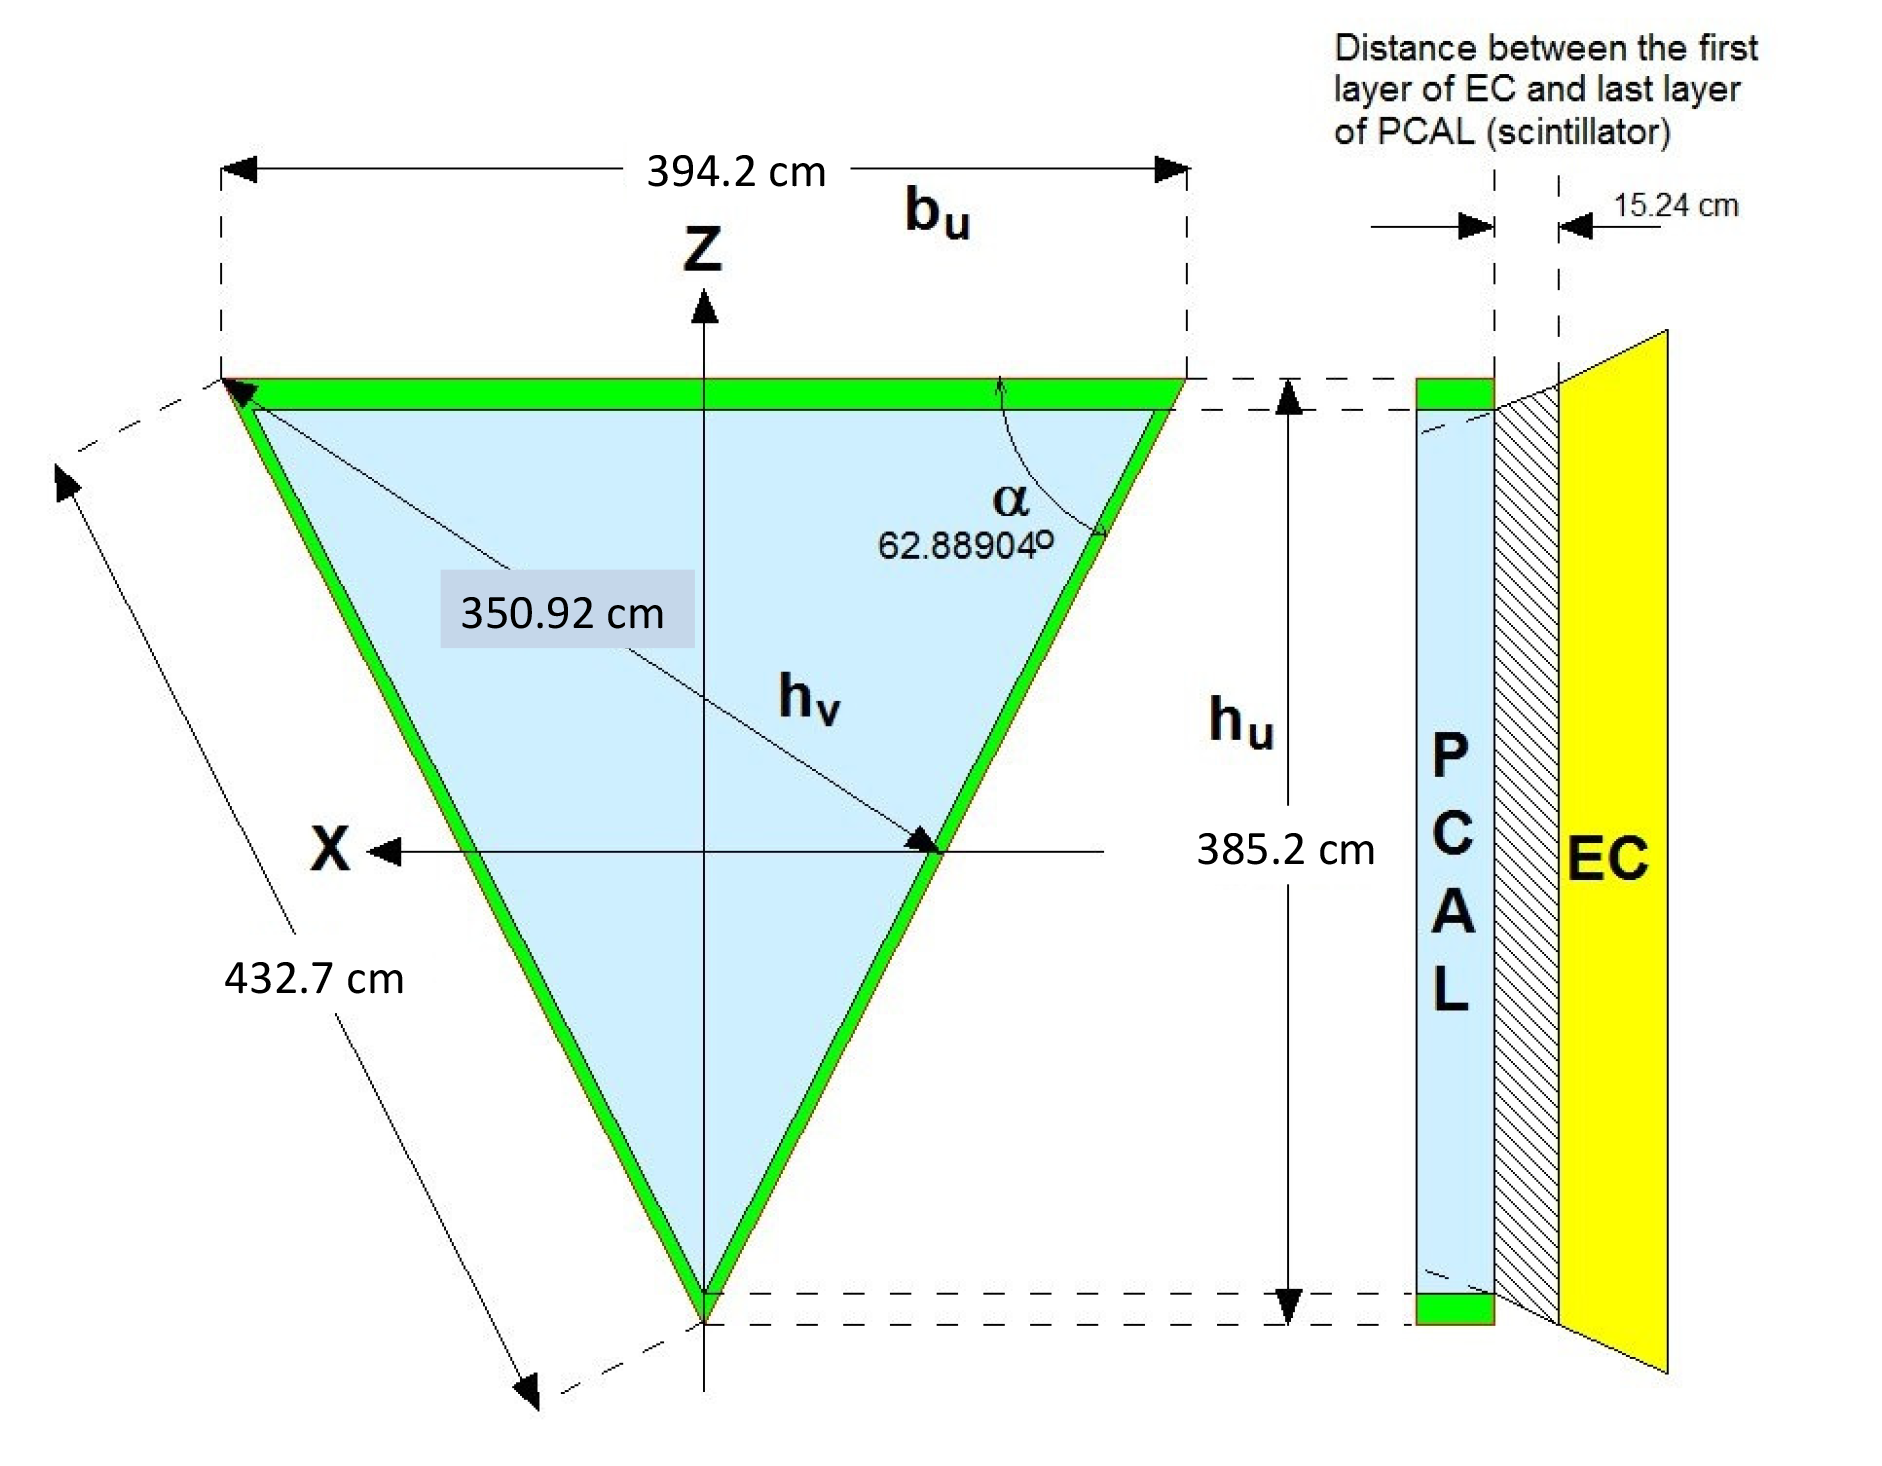
\includegraphics[width= 6in, keepaspectratio = true]{Pcal_geom_fig1}
    \caption{This diagram demonstrates the dimensions of the PCAL unit. This figure has been taken directly from the PCAL geometry note\cite{bib:geomnote}.}
    \label{fig:geomfig1}
\end{figure}

The PCAL box encapsulates layers of scintillator strips and lead sheets. 
Between each lead sheet there are three different orientations of scintillating strips. 
These orientations are described as the u, v, and w layers. 
Each layer is parallel with one side of the PCAL box. 
The sequencing of the lead sheet, u layer, v layer, and w layer is repeated five times within each sector of the PCAL unit. 
This results in fifteen layers of scintillator strips.
Each repeating layer signal is coupled to the same PMT, and  is not able to separate five different signals. 
A uvw view of the PCAL can be seen in figure \ref{fig:geomfig5}.


\begin{figure}[h]
    \centering
    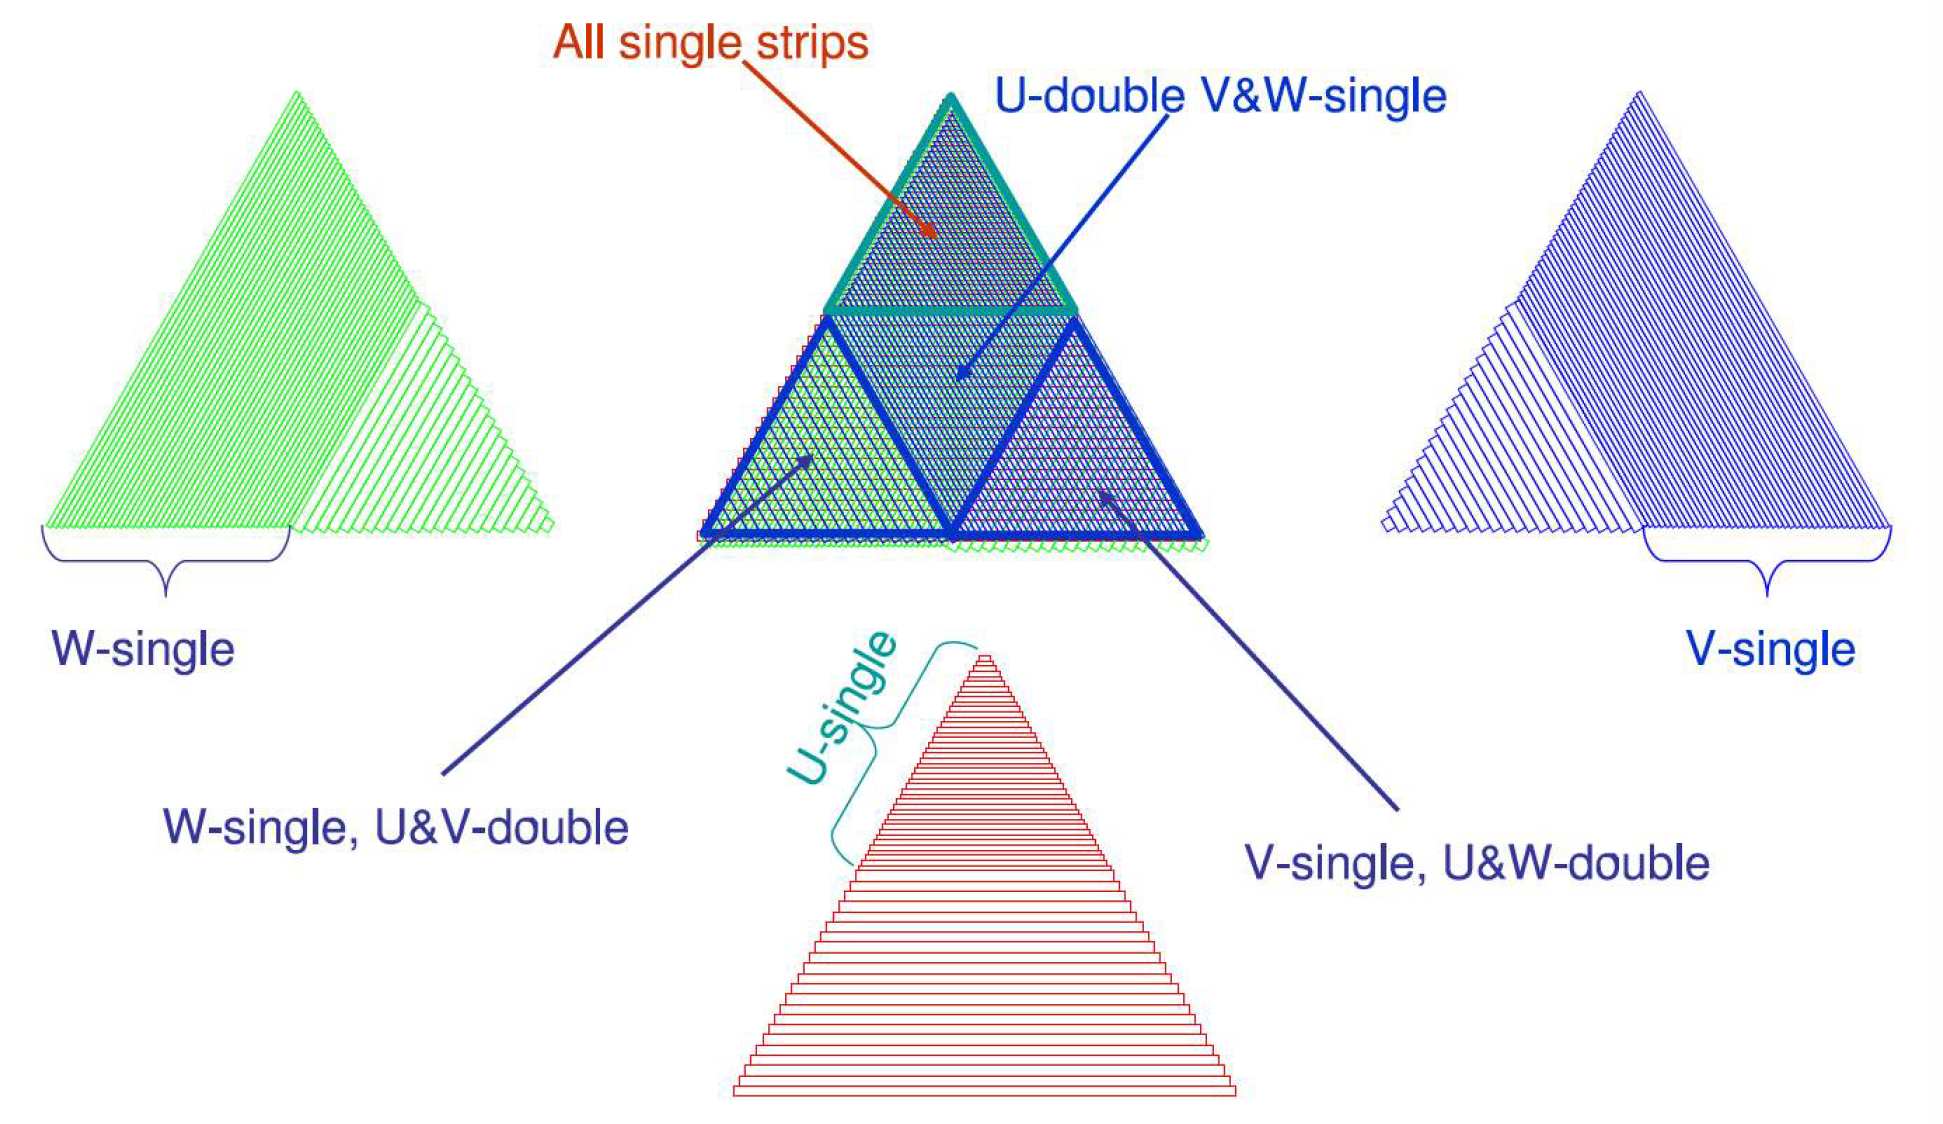
\includegraphics[width= 6in, keepaspectratio = true]{Pcal_geom_fig5}
    \caption{This is a schematic of how each orientation of scintillator is laid out. This figure is also taken directly from the PCAL geometry note\cite{bib:geomnote}.}
    \label{fig:geomfig5}
\end{figure}

There are 84 u strips, 77 v strips, and 77 w strips in each corresponding layer. 
The last 30 u strips are grouped into pairs to be readout to one PMT. 
The first 30 v and w strips are also grouped in pairs within their respective layer.
As a consequence there is better spatial resolution at low strip numbers in the u layer and at high numbers in the v and w layers. 
This pattern of scintillators can be seen in Figure \ref{fig:geomfig5}.





